This tool is best used as an interactive and cooperative
assistant to human risk analysts, rather than a fully
automated risk discovery solution.
This human-in-the-loop approach minimizes the risk of 
any obvious mistakes (hallucinations) made by the AI model,
while still improving the speed and coverage
of the risk discovery process while reducing human biases.
The human feedback is required after every step of the
process, thus minimizing the risk of positive error 
feedback loops.
We developed AIRA with the aim of creating a tool that
could be easily integrated into risk analysis meetings,
improving collaboration of the team and the overall
effectiveness of the risk discovery process.

The workflow of AIRA can be summarized in the following steps:
\begin{enumerate}
    \setcounter{enumi}{-1}
    \item \textbf{Context Definition:} The user provides
    AIRA with the context of the project (\autoref{fig:settings}) and any relevant
    information about the company, industry, or domain (\autoref{fig:project_creation}).
    This information is used to tailor the risk analysis
    process to the specific needs of the project.
    \item \textbf{Risk Discovery:} AIRA generates a list
    of potential opportunities and threats based on the
    provided context. This list is then presented to the
    user for review. The user can accept, reject, or modify
    the suggested risks, and can also provide additional
    risks that AIRA may have missed (\autoref{fig:risk_discovery}).
    \item \textbf{Qualitative Analysis:} For each accepted
    risk, AIRA assists the user in performing a qualitative
    analysis by suggesting potential impacts and likelihoods.
    The user is presented with two editable graphs that
    visualize the impact and likelihood of each risk.
    The user can adjust the graphs as needed to reflect
    their assessment of the risk. Then, a risk score
    threshold can be set to filter out low-priority risks (\autoref{fig:qualitative_analysis}).
    \item \textbf{Planning:} Finally, AIRA helps the user
    to develop contingency and fallback plans for the
    high-priority risks. AIRA suggests possible plans
    based on one of these strategies: avoid, mitigate,
    transfer, or accept for threats; exploit, enhance,
    share, or accept for opportunities. The user can
    review and modify the suggested plans as needed (\autoref{fig:planning}).
    \item \textbf{Overview:} At the end of the process,
    AIRA provides a comprehensive overview of all identified
    risks, their qualitative analysis, and the associated
    contingency and fallback plans. This overview can be
    exported for documentation and further review (\autoref{fig:download}).
\end{enumerate}

\begin{figure}[H]
    \centering
    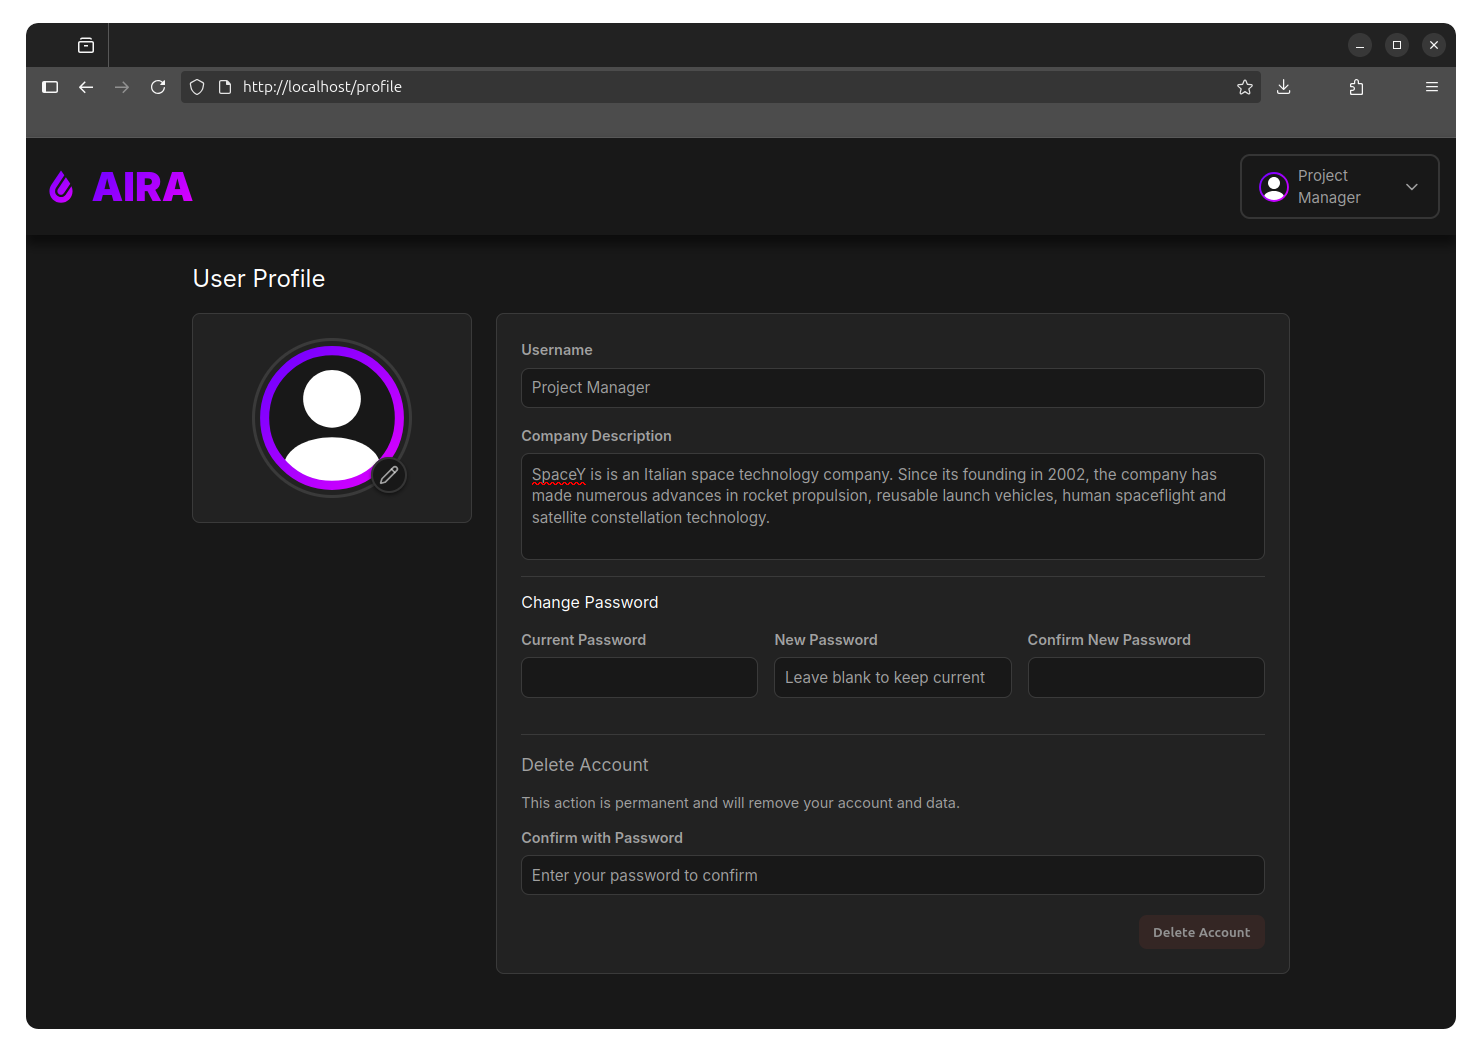
\includegraphics[width=0.8\textwidth]{figures/screenshots/settings.png}
    \caption{AIRA Account Settings interface. Setting 
    the Company Description is part of the Context 
    Definition step, and helps AIRA tailor its risk 
    analysis to the specific needs of the user's 
    organization.}
    \label{fig:settings}
\end{figure}

\begin{figure}[H]
    \centering
    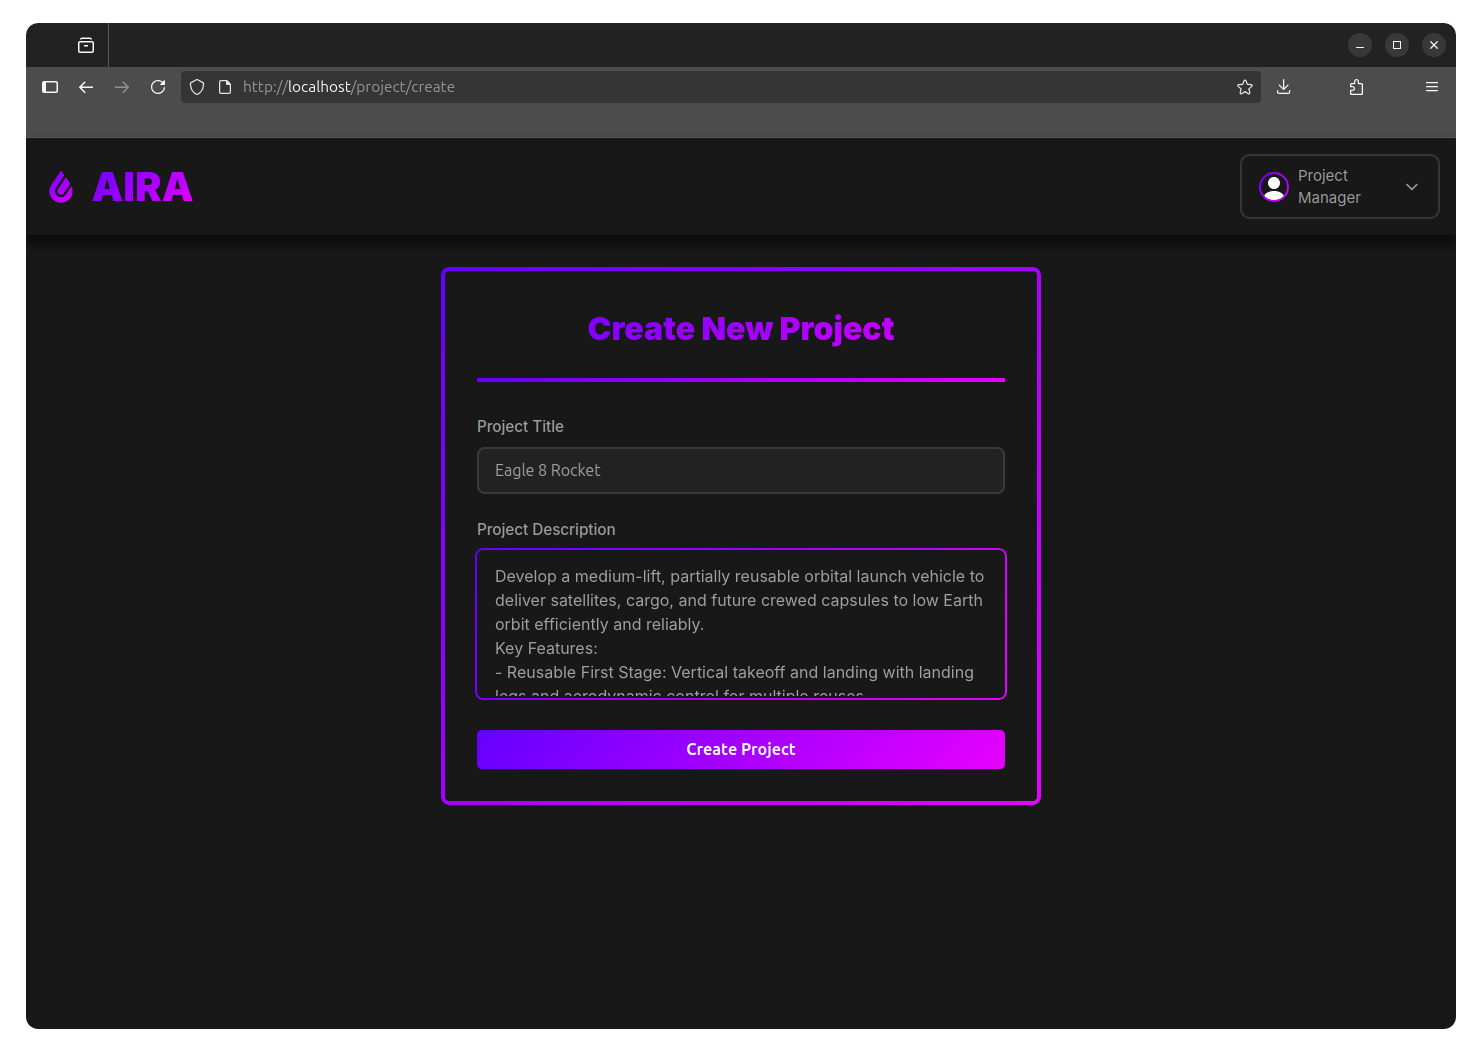
\includegraphics[width=0.8\textwidth]{figures/screenshots/project_creation.png}
    \caption{AIRA Project Creation interface. Here the 
    user can provide specific details about the project
    to be analyzed, further refining the context for
    AIRA's risk discovery process.}
    \label{fig:project_creation}
\end{figure}

\begin{figure}[H]
    \centering
    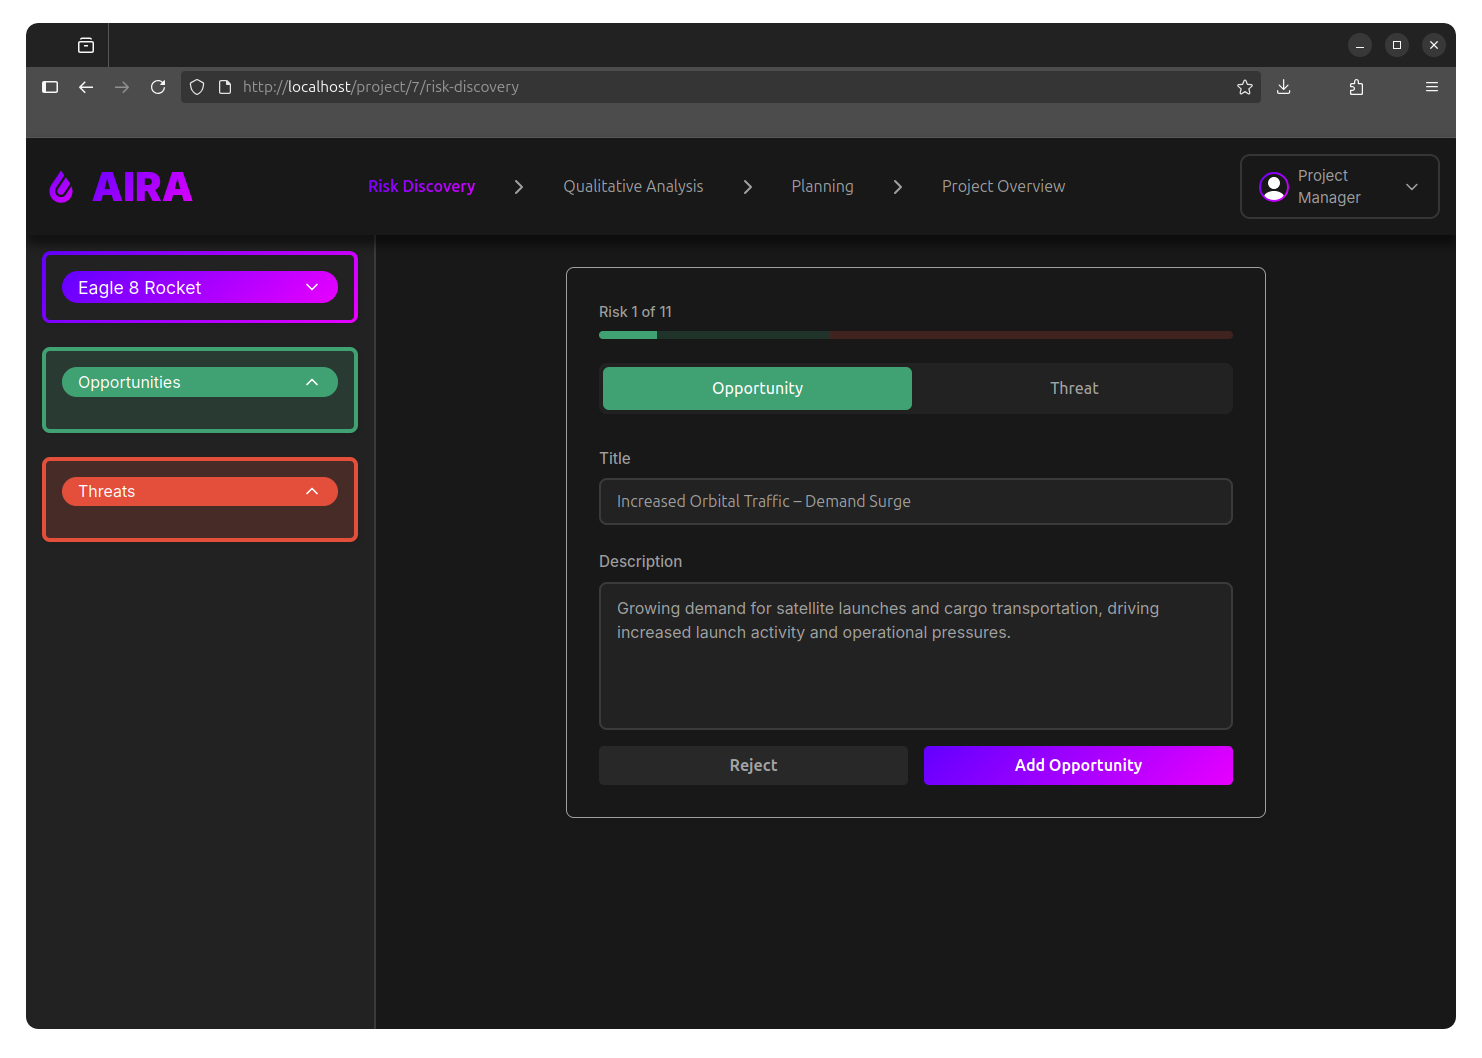
\includegraphics[width=0.8\textwidth]{figures/screenshots/risk_discovery.png}
    \caption{AIRA Risk Discovery interface. Here, AIRA
    presents the user with a list of potential risks
    identified based on the provided context.}
    \label{fig:risk_discovery}
\end{figure}

\begin{figure}[H]
    \centering
    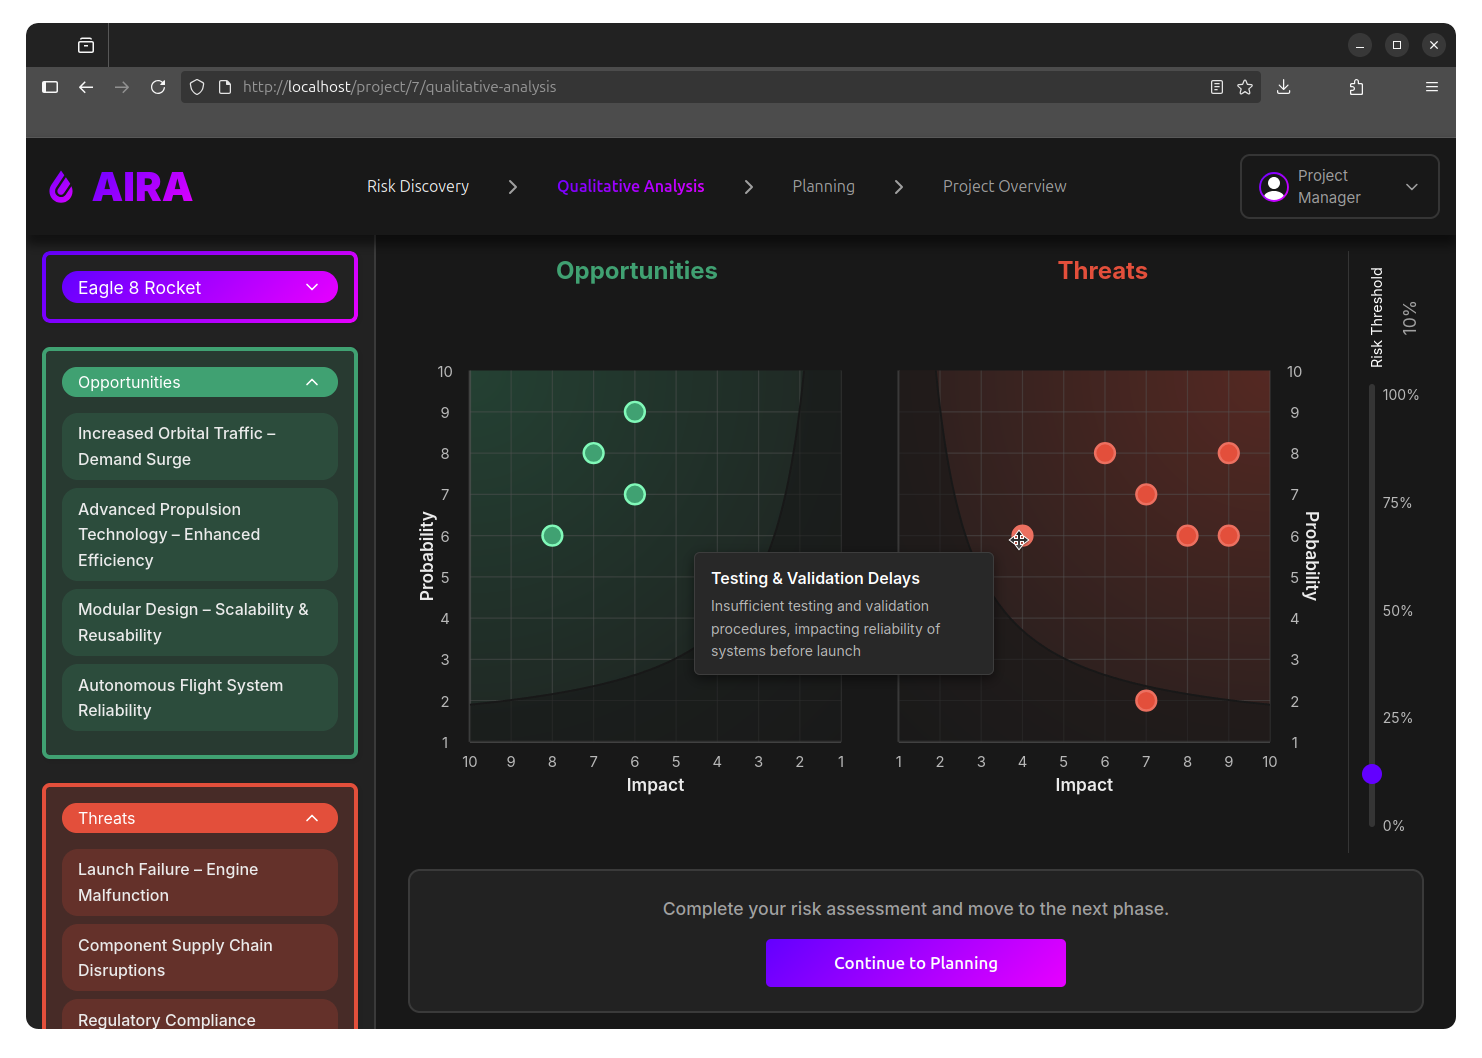
\includegraphics[width=0.8\textwidth]{figures/screenshots/qualitative_analysis.png}
    \caption{AIRA Qualitative Analysis interface. Here,
    the user can review and adjust the impact and
    likelihood assessments for each identified risk.}
    \label{fig:qualitative_analysis}
\end{figure}

\begin{figure}[H]
    \centering
    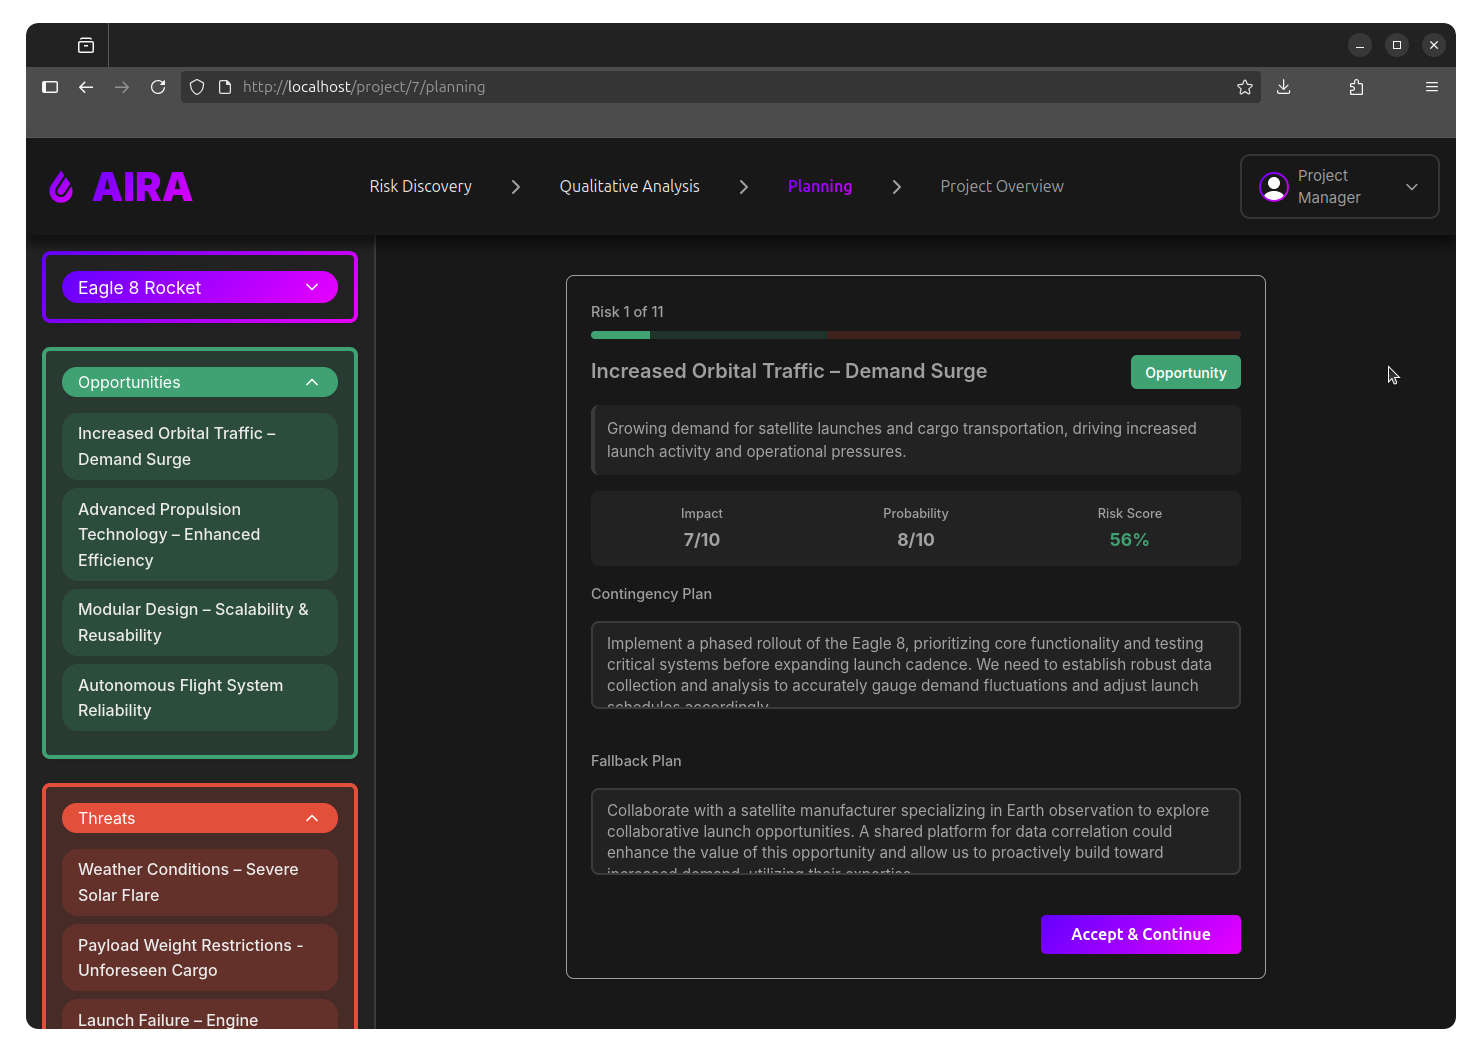
\includegraphics[width=0.8\textwidth]{figures/screenshots/planning.png}
    \caption{AIRA Planning interface. Here, AIRA
    suggests contingency and fallback plans for
    high-priority risks, which the user can review
    and modify as needed.}
    \label{fig:planning}
\end{figure}

\begin{figure}[H]
    \centering
    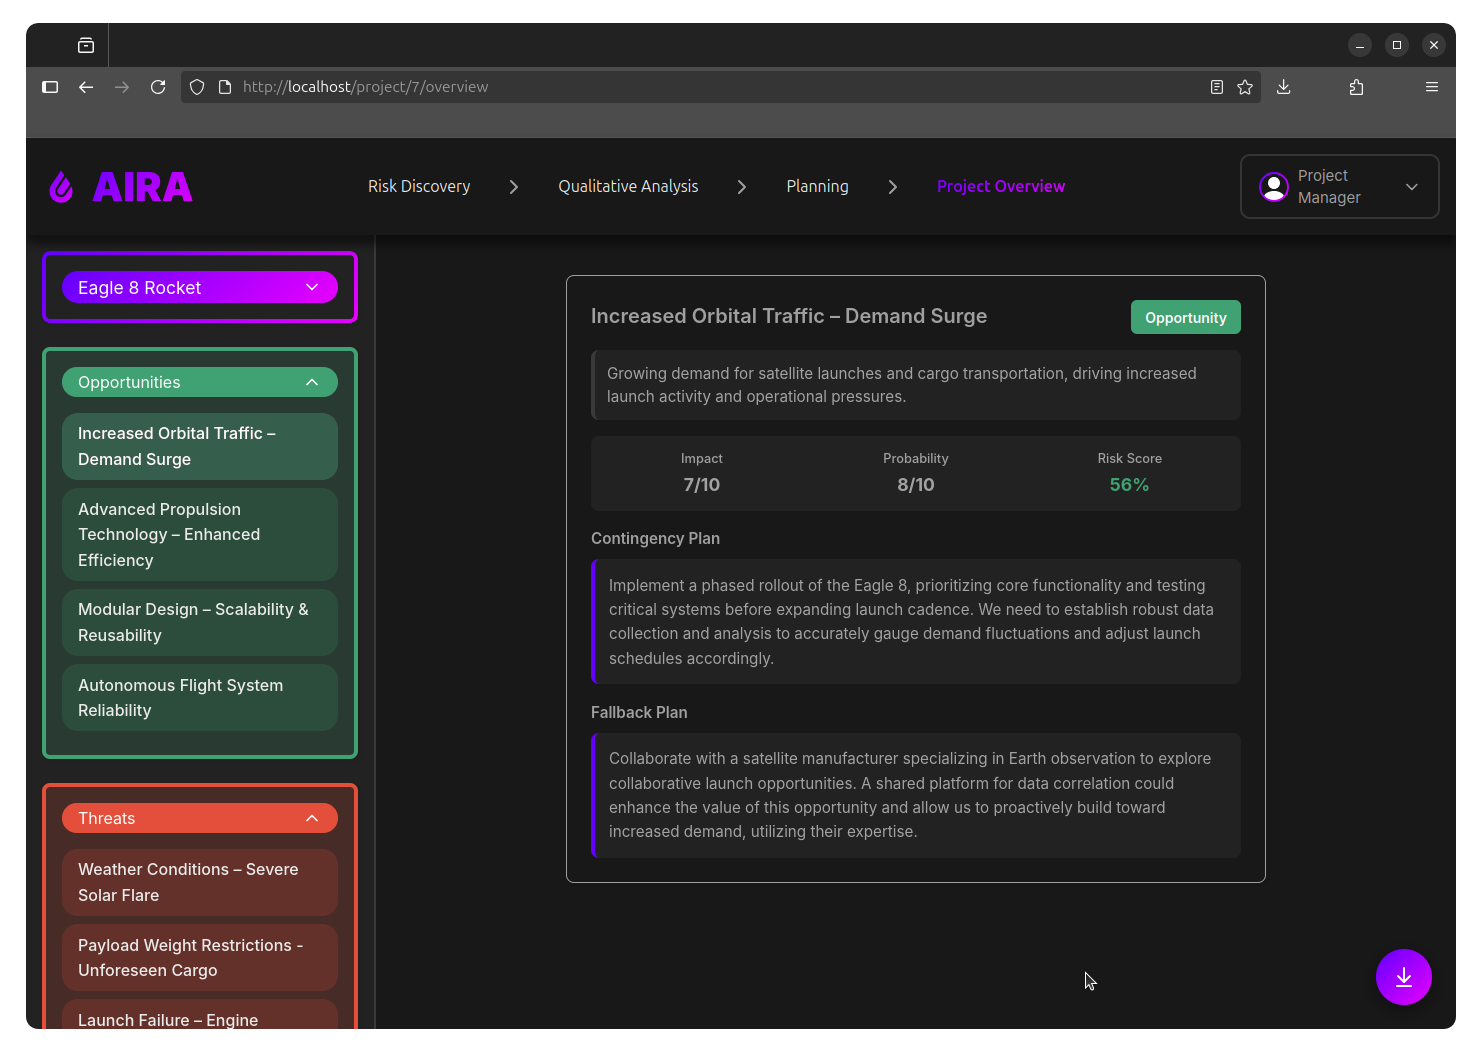
\includegraphics[width=0.8\textwidth]{figures/screenshots/overview.png}
    \caption{AIRA Overview interface. Here, the user
    can see a comprehensive summary of all identified
    risks, their qualitative analysis, and the
    associated contingency and fallback plans.}
    \label{fig:overview}
\end{figure}

\begin{figure}[H]
    \centering
    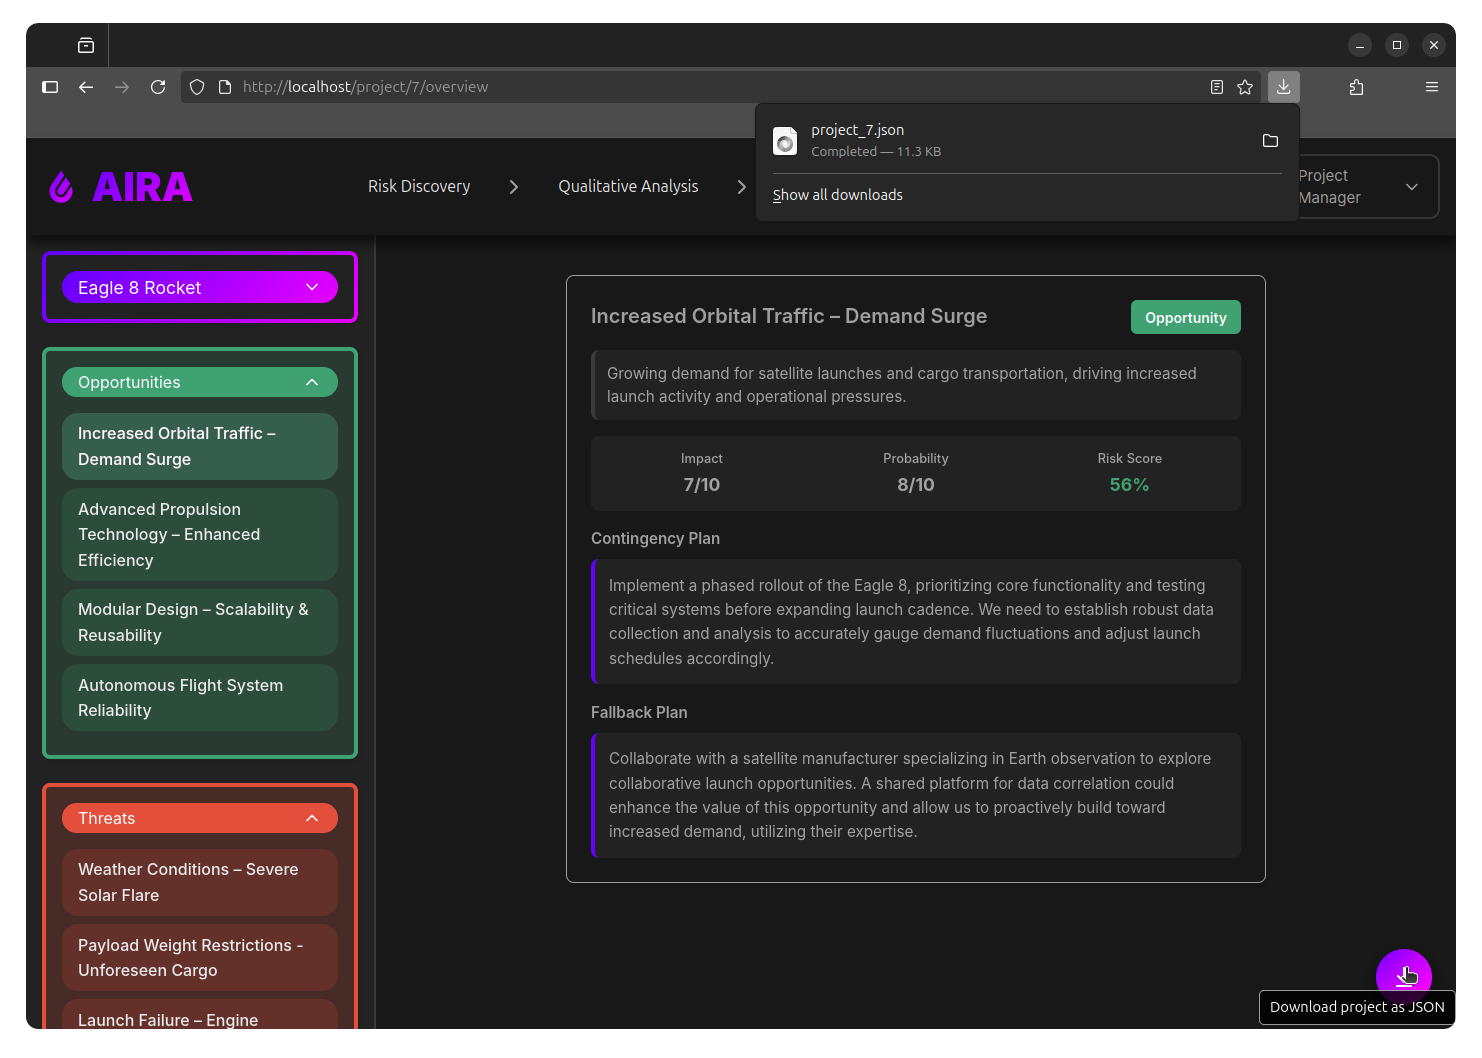
\includegraphics[width=0.8\textwidth]{figures/screenshots/download.png}
    \caption{AIRA Download feature. The user can export
    the comprehensive risk analysis report for
    documentation and further review by clicking
    the "Download" button.}
    \label{fig:download}
\end{figure}